\documentclass[tikz,border=4pt]{standalone}
\usepackage{pgfplots}
\pgfplotsset{compat=1.18}
\definecolor{argblue}{RGB}{26,79,138}
\definecolor{apsorange}{RGB}{232,119,34}
\begin{document}
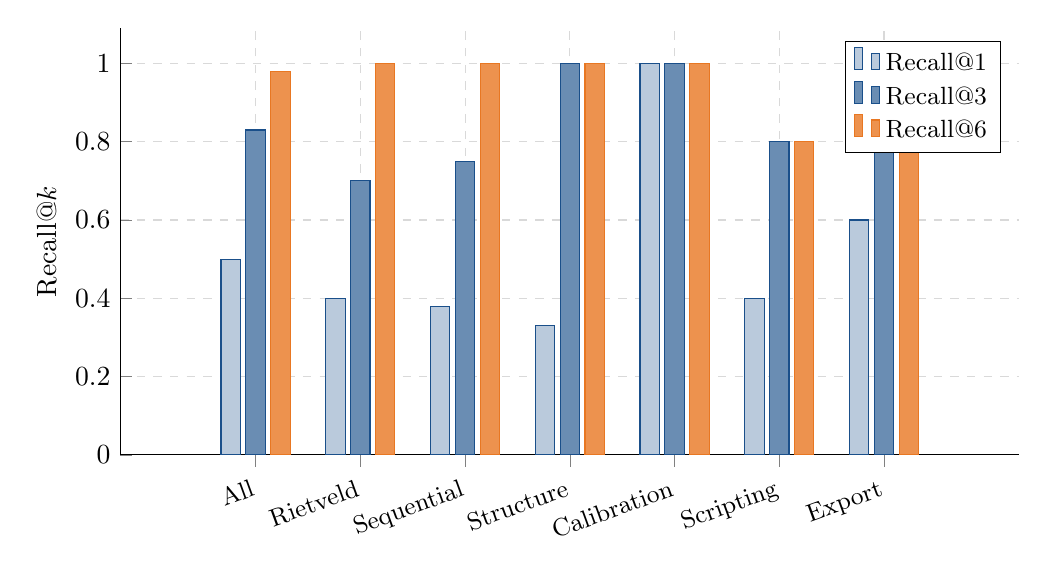
\begin{tikzpicture}
\begin{axis}[
  ybar, width=13cm, height=7cm, bar width=7pt,
  ylabel={Recall@$k$},
  ymin=0, ymax=1.09,
  ytick={0,0.2,0.4,0.6,0.8,1.0},
  xtick={1,2,3,4,5,6,7},
  xticklabels={All,Rietveld,Sequential,Structure,Calibration,Scripting,Export},
  xticklabel style={font=\small, rotate=20, anchor=north east},
  xmin=0.3, xmax=7.7,
  legend style={at={(0.98,0.97)}, anchor=north east, font=\small},
  axis lines*=left, enlarge x limits=0.08,
  grid=major, grid style={dashed,gray!30},
]
\addplot[fill=argblue!30, draw=argblue] coordinates
  {(1,0.50)(2,0.40)(3,0.38)(4,0.33)(5,1.00)(6,0.40)(7,0.60)};
\addplot[fill=argblue!65, draw=argblue] coordinates
  {(1,0.83)(2,0.70)(3,0.75)(4,1.00)(5,1.00)(6,0.80)(7,0.80)};
\addplot[fill=apsorange!80, draw=apsorange] coordinates
  {(1,0.98)(2,1.00)(3,1.00)(4,1.00)(5,1.00)(6,0.80)(7,1.00)};
\legend{Recall@1, Recall@3, Recall@6}
\end{axis}
\end{tikzpicture}
\end{document}
